\section{Requirements Document}
\subsection{Original Document}

\includepdf[pages=-, frame=true, scale=0.95]{02-requirementsdoc/group-design-requirements.pdf}

\subsection{Additions}
\subsubsection{Final Revision Document}
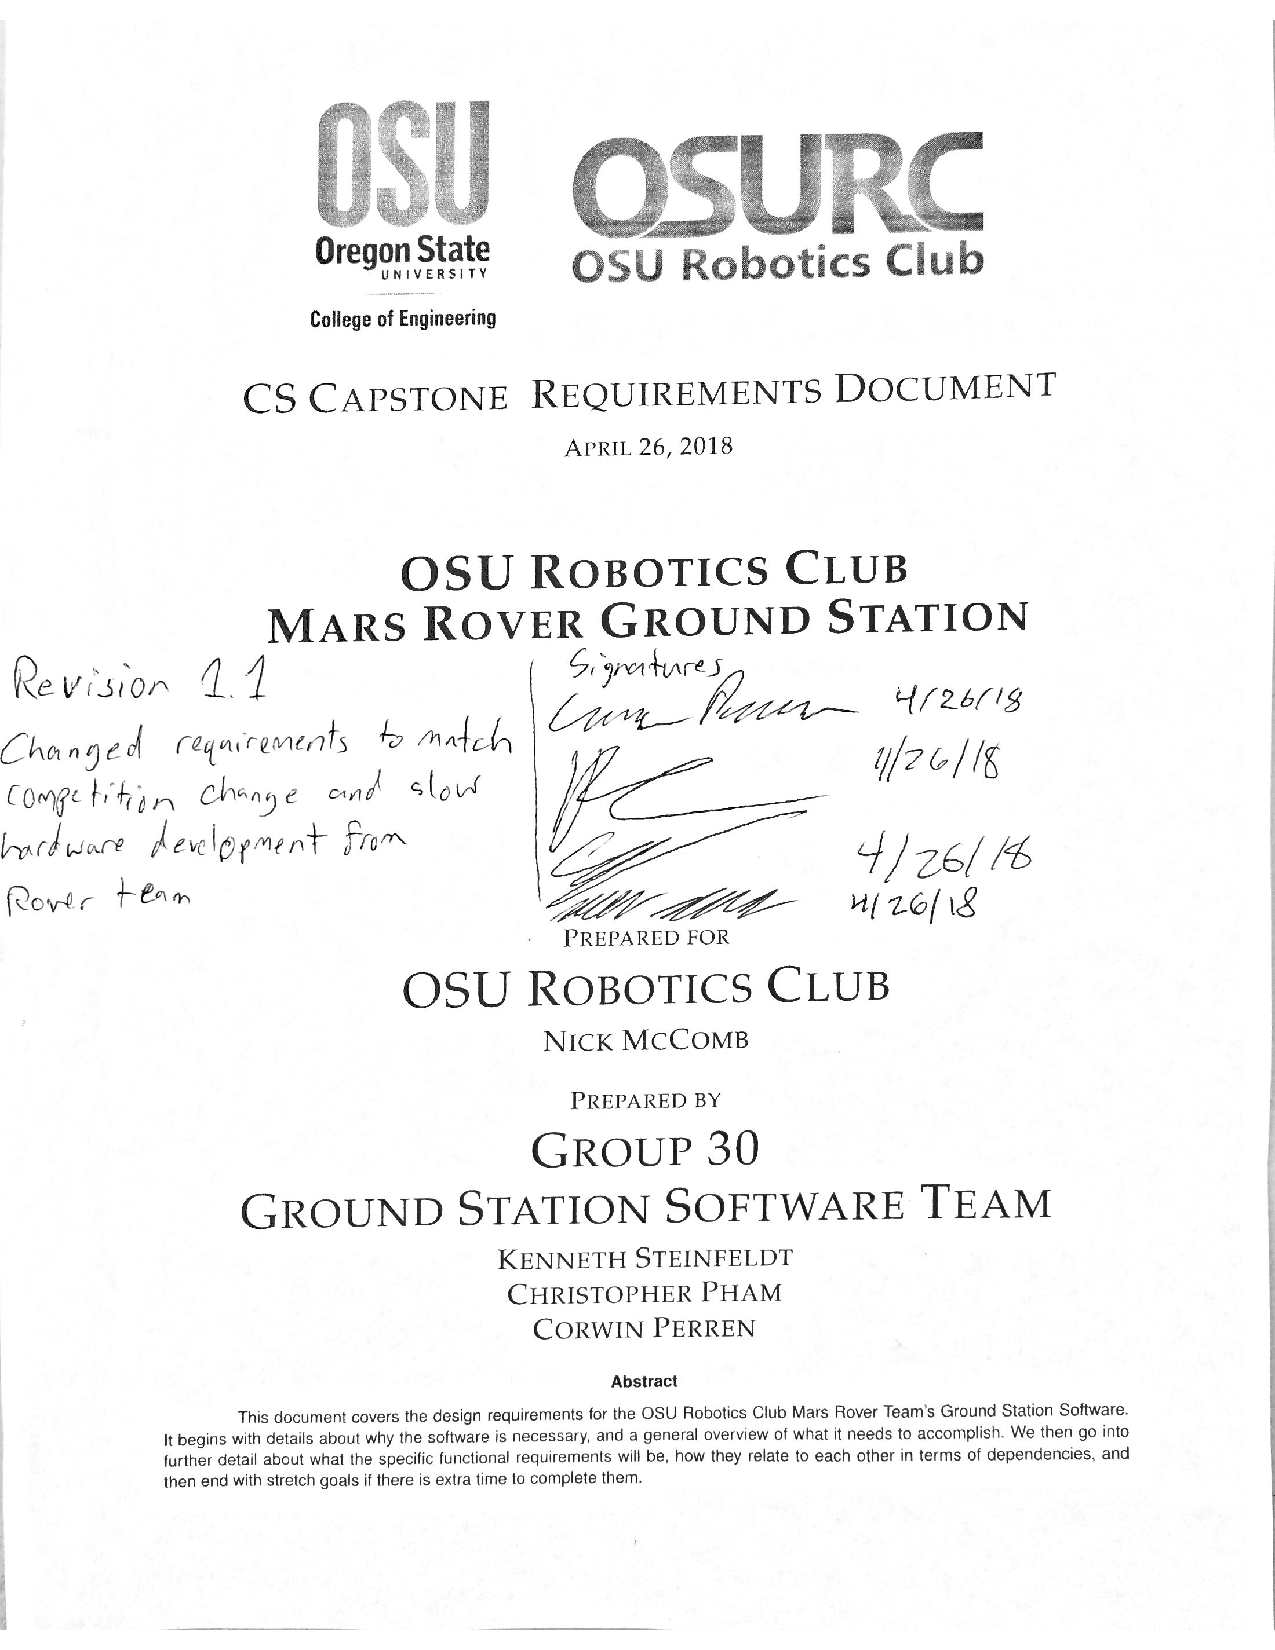
\includepdf[pages=-, frame=true, scale=0.95]{02-requirementsdoc/cs_group30_design_requirements_revision1_1.pdf}

\subsubsection{Description of Changes}
Version 1.1 of document was approved by all team members and stakeholder on 4/26/2018.

\begin{itemize}
\item Edited descriptions of competition from University Rover Challenge to Canadian International Rover Challenge
	\begin{itemize}
	\item The Mars Rover team changed competitions, so we updated the document to reflect this
	\end{itemize}
    
\item Removed user story for manual video quality adjustment
	\begin{itemize}
	\item Our team implemented automatic quality adjustment, so manual adjustment was no longer necessary
	\end{itemize}
    
\item Removed user story about easily seeing when an autonomous run has completed
	\begin{itemize}
	\item The new Rover competition does not require this display element
	\end{itemize}
    
\item Removed user story about needing to view live logs
	\begin{itemize}
	\item Log viewing was determined to not be needed as there would be too many logs to sort through in a short amount of time
	\end{itemize}
    
\item Removed user story about seeing network latency (round trip time)
	\begin{itemize}
	\item The network connection percentage was determined to be correlated with this value enough that this redundant element was not needed
	\end{itemize}

\item Added constraint that the GUI software must have placeholder for GUI elements and software features that can not be completed due to waiting on Rover team progress
	\begin{itemize}
	\item Our team encountered many situations where we could not continue development due to lack of hardware/software on Rover
    \item This new constraint allows us to still meet requirements if the bottleneck is the Rover team
	\end{itemize}
    
\item Changed functional requirement for joystick statuses so that the SpaceNav mouse had its own requirement
	\begin{itemize}
	\item The team changed to a SpaceNav mouse earlier in the year and it was determined that an individual readout for this input device would be convenient
	\end{itemize}
    
\item Changed functional requirement for battery status to battery voltage
	\begin{itemize}
	\item The battery status value was determined to be most useful as a voltage, rather than a percentage estimate
	\end{itemize}
    
\item Removed functional requirement for Rover voltage statuses
	\begin{itemize}
	\item The Rover design changed so that only the battery voltage is measured
	\end{itemize}
    
\item Changed functional requirement for bogie connection statuses to be individual wheel statuses
	\begin{itemize}
	\item The Rover software team got individual status information for each wheel, rather than a two wheel bogie group, and requested this change
	\end{itemize}
    
\item Removed functional requirement for Rover network round trip time
	\begin{itemize}
	\item The network connection percentage was determined to be correlated with this value enough that this redundant element was not needed
	\end{itemize}
    
\item Changed functional requirement for Rover arm joystick control to SpaceNav mouse control
	\begin{itemize}
	\item The team changed to a SpaceNav mouse over a second joystick for arm control
	\end{itemize}
    
\item Removed functional requirement for way-point navigation path
	\begin{itemize}
	\item Expectations for how autonomy on the Rover would work would not easily give our team this information to display
	\end{itemize}
    
\item Changed functional requirement for the autonomy indicator so that it shows whether autonomy is active rather than when autonomy is finished
	\begin{itemize}
	\item Changing to the Canadian International Rover Challenge made the old requirement unnecessary
	\end{itemize}
    
\item Removed functional requirement for video FPS counters
	\begin{itemize}
	\item FPS counters would have been useful for manual video quality adjustment, but are no longer needed with automatic quality adjustment
	\end{itemize}
    
\item Removed functional requirement for log file viewing
	\begin{itemize}
	\item Log files were too large to usefully sort through in a short amount of time
	\end{itemize}
    
\end{itemize}

\subsection{Final Gantt Chart}
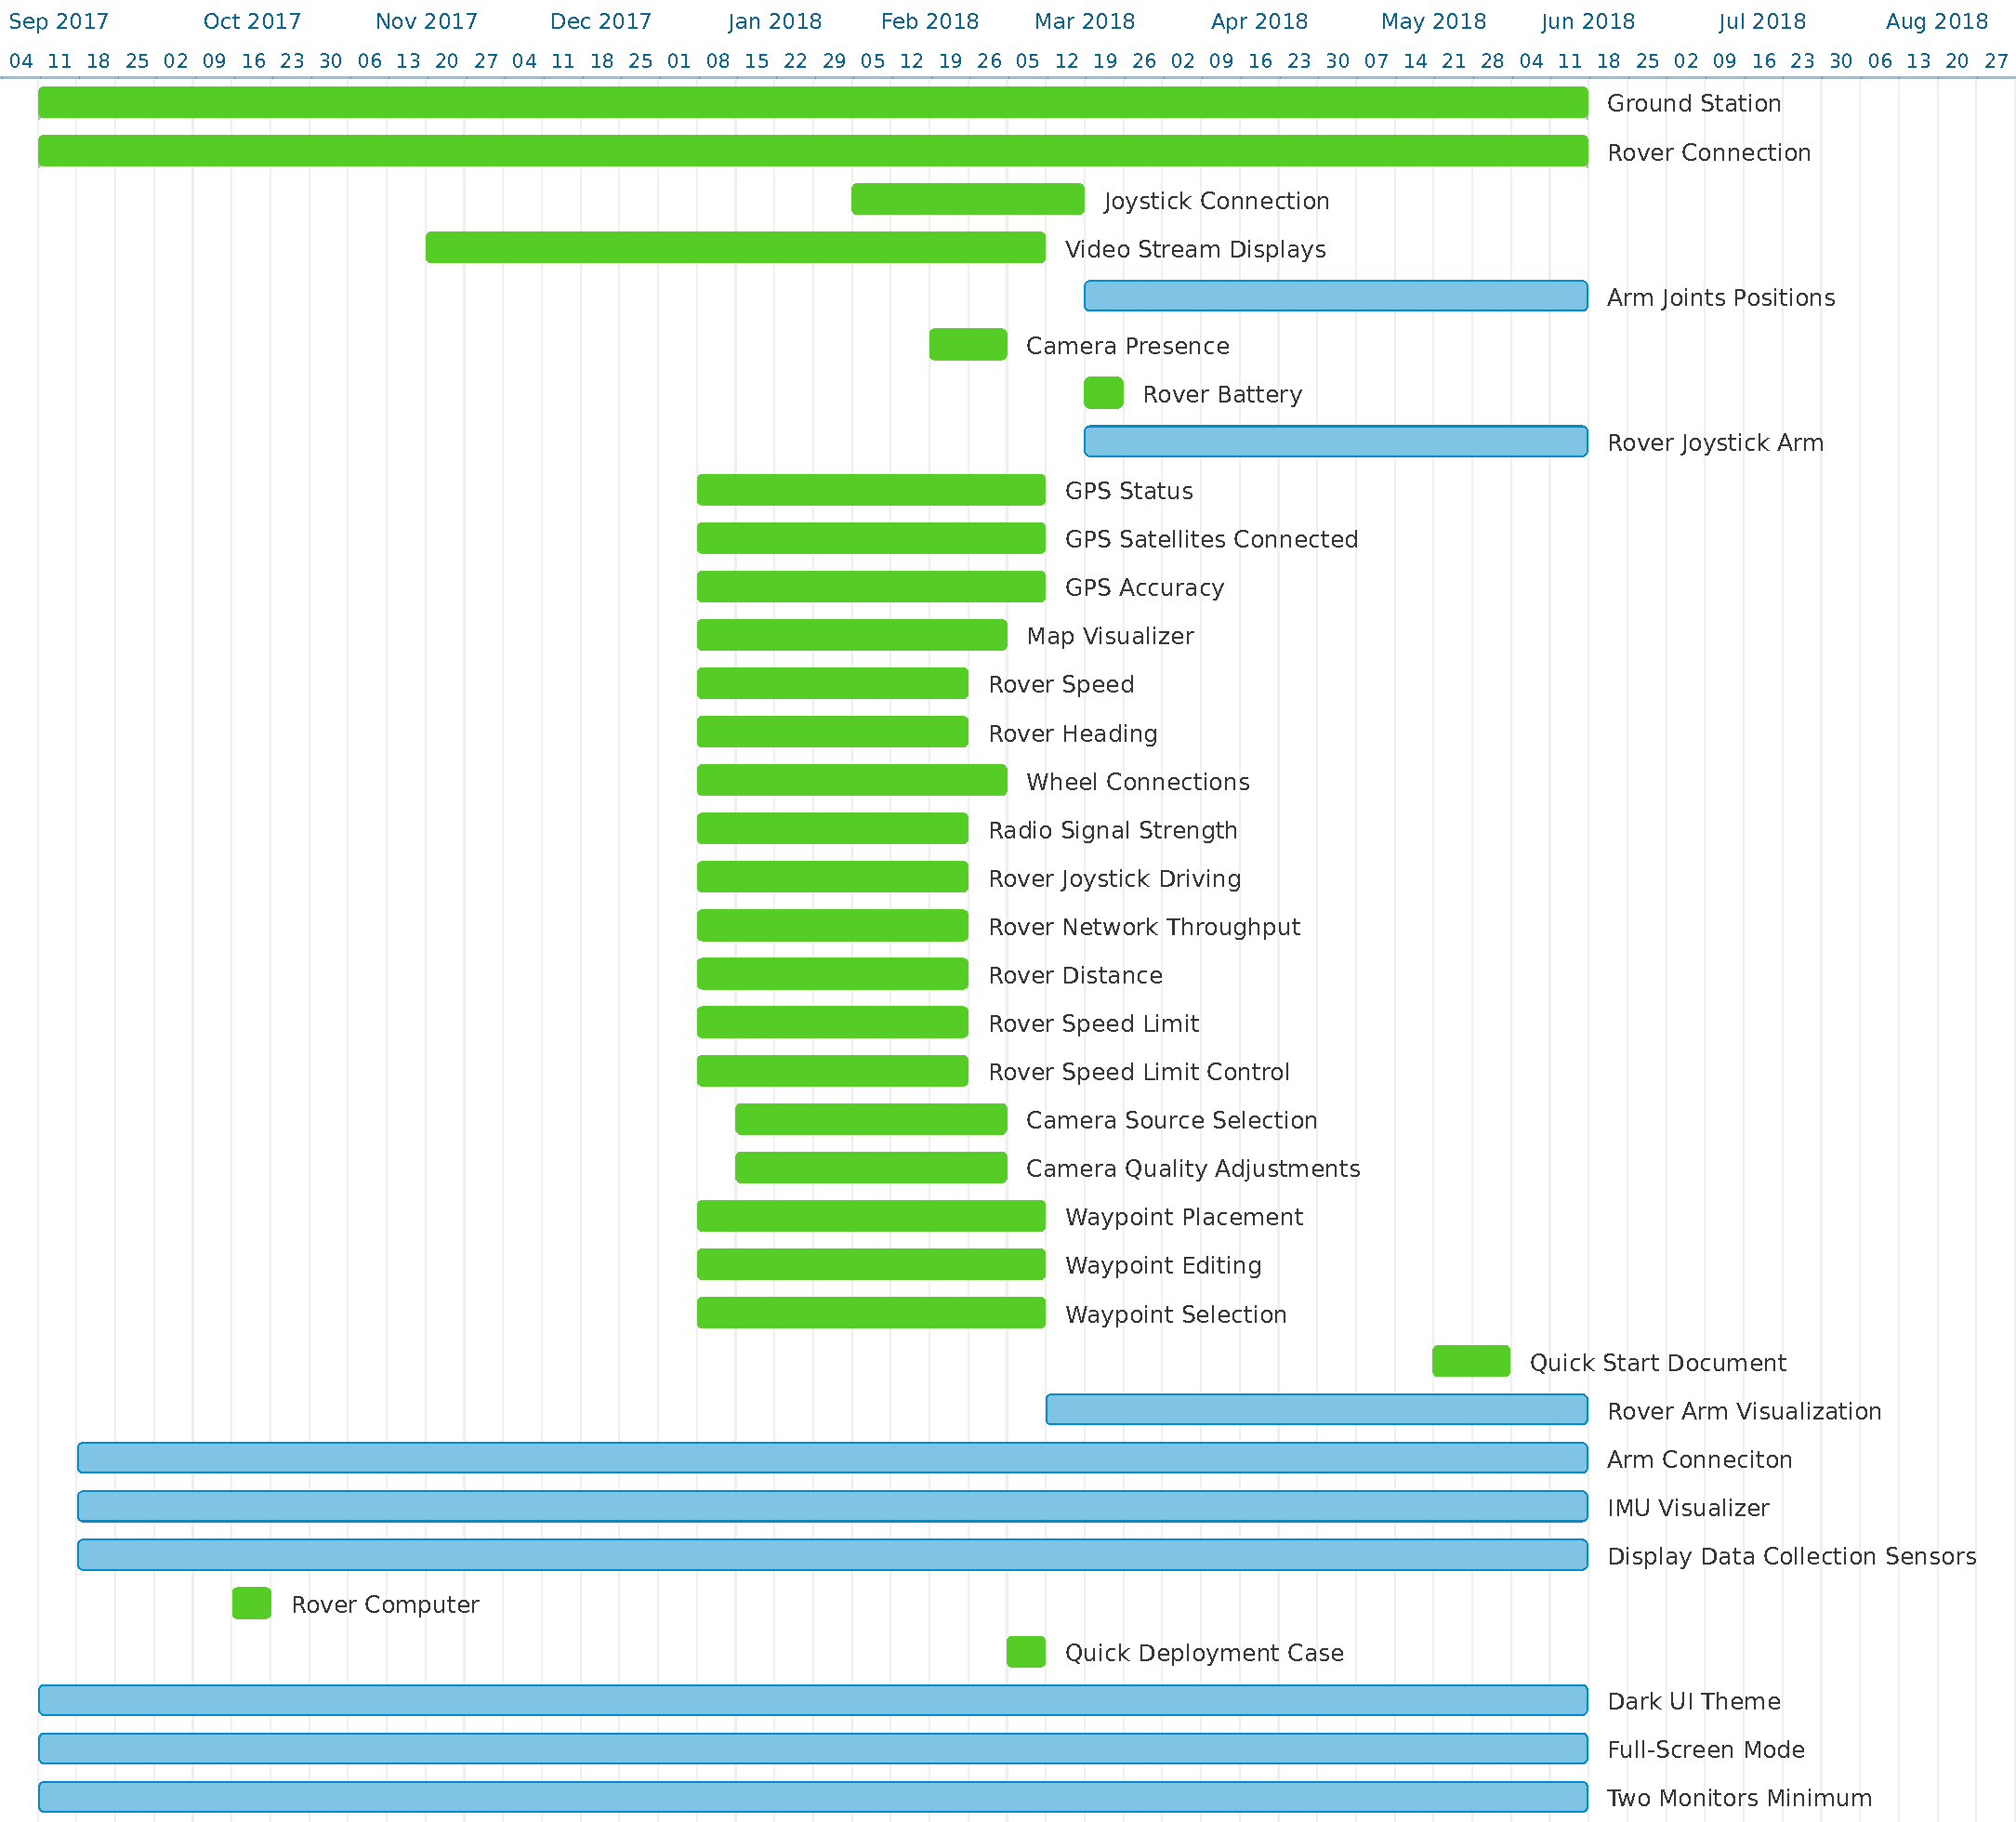
\includepdf[pages=-, frame=true, landscape, scale=0.95]{02-requirementsdoc/final_gantt.pdf}